\documentclass[11pt,a4paper]{report}

\usepackage[T1]{fontenc}
\usepackage[utf8]{inputenc}
\usepackage{lmodern}
\usepackage[margin=2.2cm,top=2.6cm,bottom=2.8cm]{geometry}
\usepackage{amsmath}
\usepackage{amssymb}
\usepackage[table]{xcolor}
\usepackage{booktabs}
\usepackage{array}
\usepackage{tabularx}
\usepackage{tikz}
\usetikzlibrary{positioning,calc,backgrounds}
\usepackage[most]{tcolorbox}
\usepackage{fontawesome5}
\usepackage{enumitem}
\usepackage{titlesec}
\usepackage{fancyhdr}
\usepackage{caption}
\usepackage{float}
\usepackage{hyperref}

% -------------------------------------------------------------------
% Palette
% -------------------------------------------------------------------
\definecolor{navy}{HTML}{13293D}
\definecolor{teal}{HTML}{1B998B}
\definecolor{slategray}{HTML}{54626F}
\definecolor{amber}{HTML}{C97A2B}
\definecolor{palebg}{HTML}{F2F5F7}

\hypersetup{
  colorlinks=true,
  linkcolor=navy,
  citecolor=navy,
  urlcolor=teal,
  pdftitle={Network Topography and Routing Guide},
  pdfauthor={Meridian Dynamics Network Engineering}
}

% -------------------------------------------------------------------
% Spacing / typography
% -------------------------------------------------------------------
\setlength{\parindent}{0pt}
\setlength{\parskip}{0.55em}
\renewcommand{\arraystretch}{1.25}

\titleformat{\chapter}[hang]
  {\normalfont\huge\bfseries\color{navy}}
  {\thechapter}
  {18pt}
  {\huge\bfseries\color{navy}}
  [\vspace{2pt}{\color{teal}\titlerule[1.4pt]}\vspace{6pt}]
\titlespacing*{\chapter}{0pt}{0pt}{16pt}

\titleformat{\section}
  {\normalfont\Large\bfseries\color{navy}}{\thesection}{9pt}{}
\titlespacing*{\section}{0pt}{16pt}{6pt}

\titleformat{\subsection}
  {\normalfont\large\bfseries\color{slategray}}{\thesubsection}{8pt}{}
\titlespacing*{\subsection}{0pt}{10pt}{4pt}

\setlength{\headheight}{14.5pt}
\pagestyle{fancy}
\fancyhf{}
\fancyhead[L]{\small\color{slategray}Meridian Dynamics --- Network Engineering}
\fancyhead[R]{\small\color{slategray}\leftmark}
\fancyfoot[C]{\small\color{slategray}\thepage}
\renewcommand{\headrulewidth}{0.6pt}
\renewcommand{\footrulewidth}{0pt}
\renewcommand{\headrule}{{\color{teal}\hrule height\headrulewidth}}

\fancypagestyle{plain}{%
  \fancyhf{}
  \fancyfoot[C]{\small\color{slategray}\thepage}
  \renewcommand{\headrulewidth}{0pt}
}

% -------------------------------------------------------------------
% Callout boxes
% -------------------------------------------------------------------
\newtcolorbox{designnote}[1][]{%
  colback=navy!5, colframe=navy, boxrule=0.6pt, arc=2pt,
  left=7pt, right=7pt, top=5pt, bottom=5pt,
  fonttitle=\bfseries\color{white}, coltitle=white,
  colbacktitle=navy,
  title={\faInfoCircle\ Design Principle},#1
}

\newtcolorbox{warnbox}[1][]{%
  colback=amber!8, colframe=amber, boxrule=0.6pt, arc=2pt,
  left=7pt, right=7pt, top=5pt, bottom=5pt,
  fonttitle=\bfseries\color{white}, coltitle=white,
  colbacktitle=amber,
  title={\faExclamationTriangle\ Operational Warning},#1
}

\newtcolorbox{factbox}[1][]{%
  colback=teal!6, colframe=teal!70!black, boxrule=0.6pt, arc=2pt,
  left=7pt, right=7pt, top=5pt, bottom=5pt,
  fonttitle=\bfseries\color{white}, coltitle=white,
  colbacktitle=teal!70!black,
  title={\faCheckCircle\ At a Glance},#1
}

% Table header helper (used inline, no @ in name)
\newcommand{\thd}[1]{\textcolor{white}{\textbf{#1}}}

\begin{document}

% =====================================================================
% TITLE PAGE
% =====================================================================
\begin{titlepage}
\centering
\vspace*{0.8cm}
{\color{teal}\rule{\linewidth}{2.2pt}}\\[0.45cm]
{\Huge\bfseries\color{navy} Network Topography \& Routing Guide}\\[0.35cm]
{\Large\color{slategray} Enterprise Campus \& Data Center Fabric --- Design Reference}\\[0.5cm]
{\color{teal}\rule{\linewidth}{2.2pt}}\\[1.6cm]

{\LARGE\bfseries\color{navy} Meridian Dynamics}\\[0.25cm]
{\large\color{slategray} Network Engineering \& Infrastructure Group}\\[2.0cm]

\begin{minipage}{0.72\linewidth}
\centering
\renewcommand{\arraystretch}{1.4}
\rowcolors{2}{palebg}{white}
\begin{tabularx}{\linewidth}{@{}l X@{}}
\rowcolor{navy}
\thd{Document Property} & \thd{Value} \\
Document Owner        & Network Engineering --- Core Infrastructure Team \\
Version                & 4.2 \\
Status                 & Approved for Production Use \\
Effective Date         & March 3, 2026 \\
Review Cycle           & Semiannual, or upon topology change \\
Classification         & Internal --- Distribution restricted \\
\end{tabularx}
\end{minipage}

\vfill
{\small\color{slategray} Prepared by Elena Cho, Principal Network Architect \\
Approved by Marcus Webb, Director of Infrastructure \\[0.3cm]
This document supersedes Version 4.1 (2025-09-15).}
\end{titlepage}

\tableofcontents
\newpage

% =====================================================================
\chapter{Introduction \& Design Principles}
% =====================================================================

\section{Purpose and Scope}
This guide is the authoritative reference for the physical and logical network architecture
of Meridian Dynamics' primary campus and its paired data center. It documents the routed
topology, IP addressing plan, interior and exterior routing policy, VLAN segmentation, and
high-availability mechanisms currently in production. It is intended for network engineers,
security operations staff, and infrastructure vendors performing authorized change work.

The scope covers the headquarters campus (Meridian Tower, Singapore), the primary data
center (DC-East), the disaster-recovery site (DC-West), and three regional branch offices.
It does not cover application-layer configuration, endpoint management, or the public-facing
CDN, which are documented separately by the Platform Engineering group.

\section{Design Principles}
The fabric is built around four principles that every change request is evaluated against:

\begin{itemize}[leftmargin=1.4em]
  \item \textbf{No single point of failure.} Every layer from transit circuit to access
    switch is deployed in an active/standby or active/active pair.
  \item \textbf{Deterministic addressing.} Every subnet is derived from a documented
    supernet so that any address can be traced to a site and function without querying
    a live system.
  \item \textbf{Defense in depth.} Traffic between trust zones always crosses at least one
    stateful inspection point; no zone trusts another implicitly.
  \item \textbf{Change is reversible.} Every routing and VLAN change ships with a
    pre-verified rollback step before it is scheduled.
\end{itemize}

\begin{factbox}
\begin{minipage}[t]{0.48\linewidth}
Sites in scope: \textbf{5} (HQ, DC-East, DC-West, 3 branches shown as one class)\\
Core address space: \textbf{10.0.0.0/8}\\
Interior routing: \textbf{OSPFv2}, 4 areas
\end{minipage}\hfill
\begin{minipage}[t]{0.48\linewidth}
Exterior routing: \textbf{eBGP}, dual transit, AS 65001\\
Core switching: redundant pair, MLAG\\
Firewall posture: active/standby, stateful failover
\end{minipage}
\end{factbox}

% =====================================================================
\chapter{Network Topology}
% =====================================================================

\section{Topology Overview}
The fabric follows a classic three-tier design --- core, distribution, access --- with a
dedicated security tier sitting between the Internet edge and the core. Figure~\ref{fig:topology}
shows the logical layout for the HQ campus; DC-East mirrors the same pattern with the
distribution tier replaced by top-of-rack leaf switches.

\begin{figure}[H]
\centering
\resizebox{\linewidth}{!}{%
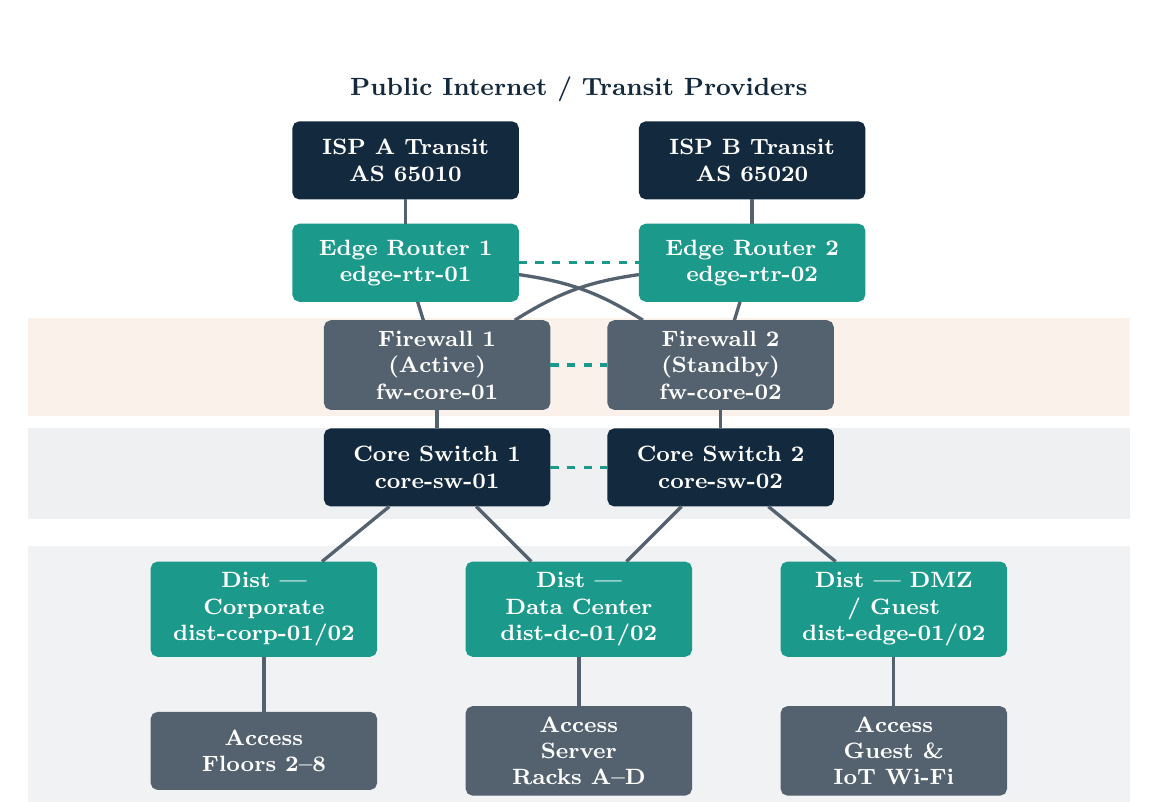
\begin{tikzpicture}[
  font=\small,
  box/.style={rectangle, rounded corners=2pt, draw=navy, very thick, fill=navy,
    text=white, text width=2.6cm, minimum height=0.95cm, align=center,
    font=\bfseries\footnotesize},
  boxalt/.style={box, draw=teal, fill=teal},
  boxlight/.style={box, draw=slategray, fill=slategray},
  link/.style={very thick, draw=slategray},
  halink/.style={very thick, dashed, draw=teal},
]

\begin{scope}[on background layer]
  \fill[amber!10] (-7.0,-3.25) rectangle (7.0,-2.0);
  \fill[navy!7]   (-7.0,-4.55) rectangle (7.0,-3.4);
  \fill[slategray!8] (-7.0,-8.3) rectangle (7.0,-4.9);
\end{scope}

\node[font=\bfseries\small, color=navy] at (0,0.9) {Public Internet / Transit Providers};

\node[box]     (isp1) at (-2.2,0)    {ISP A Transit\\AS 65010};
\node[box]     (isp2) at (2.2,0)     {ISP B Transit\\AS 65020};

\node[boxalt]  (edge1) at (-2.2,-1.3) {Edge Router 1\\edge-rtr-01};
\node[boxalt]  (edge2) at (2.2,-1.3)  {Edge Router 2\\edge-rtr-02};

\node[boxlight] (fw1) at (-1.8,-2.6) {Firewall 1 (Active)\\fw-core-01};
\node[boxlight] (fw2) at (1.8,-2.6)  {Firewall 2 (Standby)\\fw-core-02};

\node[box]     (core1) at (-1.8,-3.9) {Core Switch 1\\core-sw-01};
\node[box]     (core2) at (1.8,-3.9)  {Core Switch 2\\core-sw-02};

\node[boxalt]  (dist1) at (-4.0,-5.7) {Dist --- Corporate\\dist-corp-01/02};
\node[boxalt]  (dist2) at (0,-5.7)    {Dist --- Data Center\\dist-dc-01/02};
\node[boxalt]  (dist3) at (4.0,-5.7)  {Dist --- DMZ / Guest\\dist-edge-01/02};

\node[boxlight] (acc1) at (-4.0,-7.5) {Access\\Floors 2--8};
\node[boxlight] (acc2) at (0,-7.5)    {Access\\Server Racks A--D};
\node[boxlight] (acc3) at (4.0,-7.5)  {Access\\Guest \& IoT Wi-Fi};

\draw[link] (isp1) -- (edge1);
\draw[link] (isp2) -- (edge2);
\draw[halink] (edge1) -- (edge2);
\draw[link] (edge1) -- (fw1);
\draw[link] (edge2) -- (fw2);
\draw[link] (edge1) to[bend left=12] (fw2);
\draw[link] (edge2) to[bend right=12] (fw1);
\draw[halink] (fw1) -- (fw2);
\draw[link] (fw1) -- (core1);
\draw[link] (fw2) -- (core2);
\draw[halink] (core1) -- (core2);
\draw[link] (core1) -- (dist1);
\draw[link] (core1) -- (dist2);
\draw[link] (core2) -- (dist2);
\draw[link] (core2) -- (dist3);
\draw[link] (dist1) -- (acc1);
\draw[link] (dist2) -- (acc2);
\draw[link] (dist3) -- (acc3);
\end{tikzpicture}%
}
\caption{Logical topology of the HQ campus fabric, including the Internet edge and security tier.}
\label{fig:topology}
\end{figure}

\noindent
\tikz\fill[navy] (0,0) rectangle (0.32,0.32);\ Edge \& core routing/switching devices \quad
\tikz\fill[teal] (0,0) rectangle (0.32,0.32);\ Redundant, HA-paired, or distribution devices \quad
\tikz\fill[slategray] (0,0) rectangle (0.32,0.32);\ Access layer and standby links

\noindent
\tikz\fill[amber!10] (0,0) rectangle (0.32,0.32);\ Security tier \quad
\tikz\fill[navy!7] (0,0) rectangle (0.32,0.32);\ Core tier \quad
\tikz\fill[slategray!8] (0,0) rectangle (0.32,0.32);\ Distribution / access tier

\section{Site Inventory}
Table~\ref{tab:sites} lists every routed site in the fabric and its role in the overall
design. All inter-site links are encrypted point-to-point circuits terminated on the edge
routers shown in Figure~\ref{fig:topology}.

\begin{table}[H]
\centering
\rowcolors{2}{palebg}{white}
\begin{tabularx}{\linewidth}{@{}l l l X@{}}
\toprule
\rowcolor{navy}
\thd{Site} & \thd{Role} & \thd{Primary Link} & \thd{Backup Link} \\
\midrule
HQ --- Meridian Tower & Campus, user access & 2\,$\times$ 10\,Gbps dark fiber & 1\,Gbps LTE failover \\
DC-East               & Primary data center & 40\,Gbps DWDM to HQ & 10\,Gbps DWDM to DC-West \\
DC-West               & DR / warm standby   & 10\,Gbps DWDM to DC-East & 1\,Gbps Internet VPN \\
Branch --- Austin     & Regional office     & 500\,Mbps MPLS & 200\,Mbps SD-WAN broadband \\
Branch --- Lisbon     & Regional office     & 500\,Mbps MPLS & 200\,Mbps SD-WAN broadband \\
Branch --- Nairobi    & Regional office     & 200\,Mbps MPLS & 100\,Mbps SD-WAN broadband \\
\bottomrule
\end{tabularx}
\caption{Site inventory and circuit redundancy.}
\label{tab:sites}
\end{table}

% =====================================================================
\chapter{IP Addressing Plan}
% =====================================================================

\section{Address Space Summary}
All internal address space is carved from the \texttt{10.0.0.0/8} private block. Each site
receives a dedicated \texttt{/16}, and each functional zone within a site receives a
\texttt{/20} or smaller reserved range, leaving headroom for growth without renumbering.
Table~\ref{tab:supernets} is the top-level allocation; Section~\ref{sec:vlans} breaks each
site down to individual VLANs.

\begin{table}[H]
\centering
\rowcolors{2}{palebg}{white}
\begin{tabularx}{\linewidth}{@{}l l X@{}}
\toprule
\rowcolor{navy}
\thd{Site / Zone} & \thd{Supernet} & \thd{Reserved For} \\
\midrule
HQ Campus            & 10.10.0.0/16 & User, voice, and management VLANs across 8 floors \\
DC-East               & 10.20.0.0/16 & Server, storage, and out-of-band management subnets \\
DC-West (DR)          & 10.21.0.0/16 & Mirrors DC-East allocation for failover consistency \\
Branch --- Austin      & 10.30.0.0/16 & Local user and voice VLANs \\
Branch --- Lisbon      & 10.31.0.0/16 & Local user and voice VLANs \\
Branch --- Nairobi     & 10.32.0.0/16 & Local user and voice VLANs \\
DMZ / Guest (shared)  & 172.16.0.0/16 & Internet-facing services, guest Wi-Fi, IoT \\
Point-to-point links  & 192.168.0.0/22 & /31 transit links between routed devices \\
Future data center    & 10.40.0.0/16 & Reserved, unallocated \\
\bottomrule
\end{tabularx}
\caption{Top-level supernet allocation.}
\label{tab:supernets}
\end{table}

\begin{warnbox}
The \texttt{10.40.0.0/16} reservation for the planned DC-Central build-out must not be
assigned to any interim project. Two prior incidents trace back to VLANs borrowed from an
"unused" future block that later conflicted with a live migration.
\end{warnbox}

\section{VLAN and Subnet Allocation}
\label{sec:vlans}
Table~\ref{tab:vlans} enumerates every production VLAN at HQ and DC-East. Branch offices
follow the same VLAN ID scheme (100s for user, 200s for voice, 900s for management) against
their own site supernet.

\begin{table}[H]
\centering
\rowcolors{2}{palebg}{white}
\begin{tabularx}{\linewidth}{@{}l X l l l@{}}
\toprule
\rowcolor{navy}
\thd{VLAN} & \thd{Name} & \thd{Subnet} & \thd{Gateway} & \thd{DHCP Range} \\
\midrule
110 & HQ --- User Data (Floors 2--4)   & 10.10.0.0/22   & 10.10.0.1   & .0.50--.3.250 \\
120 & HQ --- User Data (Floors 5--8)   & 10.10.4.0/22   & 10.10.4.1   & .4.50--.7.250 \\
210 & HQ --- Voice / SIP               & 10.10.16.0/23  & 10.10.16.1  & .16.20--.17.250 \\
310 & HQ --- Guest Wi-Fi (in DMZ block)& 172.16.10.0/24 & 172.16.10.1 & .10.20--.10.250 \\
320 & HQ --- IoT / Building Systems    & 172.16.20.0/24 & 172.16.20.1 & .20.20--.20.250 \\
910 & HQ --- Network Management        & 10.10.250.0/24 & 10.10.250.1 & Static only \\
920 & HQ --- Security Cameras \& Badging & 10.10.251.0/24 & 10.10.251.1 & Static only \\
501 & DC-East --- Application Tier      & 10.20.1.0/24   & 10.20.1.1   & Static only \\
502 & DC-East --- Database Tier         & 10.20.2.0/24   & 10.20.2.1   & Static only \\
503 & DC-East --- Storage / iSCSI       & 10.20.3.0/25   & 10.20.3.1   & Static only \\
510 & DC-East --- Load Balancer VIPs    & 172.16.30.0/25 & 172.16.30.1 & Static only \\
930 & DC-East --- Out-of-Band Mgmt (IPMI) & 10.20.250.0/24 & 10.20.250.1 & Static only \\
\bottomrule
\end{tabularx}
\caption{VLAN and subnet allocation, HQ and DC-East (abbreviated addresses share the row's /16).}
\label{tab:vlans}
\end{table}

% =====================================================================
\chapter{Routing Architecture}
% =====================================================================

\section{Interior Routing --- OSPFv2}
The campus and data center backbone runs OSPFv2 in four areas. Area~0 is the transit
backbone linking core and distribution devices; each site's user- and server-facing
subnets are stubbed into their own totally-stubby area to keep the link-state database
small on branch routers with limited memory.

\begin{table}[H]
\centering
\rowcolors{2}{palebg}{white}
\begin{tabularx}{\linewidth}{@{}l X l@{}}
\toprule
\rowcolor{navy}
\thd{Area} & \thd{Scope} & \thd{Type} \\
\midrule
0.0.0.0 & Core-to-distribution backbone, core-sw-01/02, dist-*-01/02 & Backbone \\
0.0.0.10 & HQ campus user and voice VLANs & Totally stubby \\
0.0.0.20 & DC-East and DC-West server, storage, and OOB VLANs & Totally stubby \\
0.0.0.30 & Branch offices (Austin, Lisbon, Nairobi) & Totally stubby \\
\bottomrule
\end{tabularx}
\caption{OSPF area design.}
\label{tab:ospf}
\end{table}

\section{Exterior Routing --- BGP}
Internet transit is dual-homed with route-based failover and no default static route ---
the edge routers rely entirely on learned BGP routes so that failover behavior matches
production during a planned circuit test.

\begin{table}[H]
\centering
\rowcolors{2}{palebg}{white}
\begin{tabularx}{\linewidth}{@{}l l l X@{}}
\toprule
\rowcolor{navy}
\thd{Peer} & \thd{Peer ASN} & \thd{Local ASN} & \thd{Policy} \\
\midrule
ISP A (primary)  & 65010 & 65001 & Prefer via local preference 200; full table \\
ISP B (secondary)& 65020 & 65001 & Local preference 150; full table, AS-path prepend outbound \\
DC-West DR link  & 65001 & 65001 & iBGP over encrypted VPN; used only on DC-East failure \\
\bottomrule
\end{tabularx}
\caption{External BGP peering summary.}
\label{tab:bgp}
\end{table}

\begin{itemize}[leftmargin=1.4em]
  \item Only the summarized \texttt{10.0.0.0/8} aggregate and the DMZ \texttt{172.16.0.0/16}
    block are advertised outbound; component subnets are filtered by an outbound prefix list.
  \item Inbound, only the default route and two backup provider routes are accepted; a
    maximum-prefix limit of 25 stops an accidental full-table leak from either peer.
  \item Redistribution between BGP and OSPF is one-directional (BGP $\rightarrow$ OSPF) and
    tagged with community \texttt{65001:900} so it can never be redistributed back out.
\end{itemize}

\begin{warnbox}
Never remove the \texttt{65001:900} no-re-export community from the BGP-to-OSPF redistribution
route-map. Doing so during the 2024 edge upgrade briefly leaked internal OSPF routes toward
ISP B and triggered a maximum-prefix session reset.
\end{warnbox}

% =====================================================================
\chapter{VLAN Segmentation \& Security Zones}
% =====================================================================

\section{Trust Zone Model}
Every VLAN is assigned to exactly one of four trust zones. Traffic crossing a zone boundary
always transits a firewall context; there is no routed path between zones that bypasses
inspection.

\begin{figure}[H]
\centering
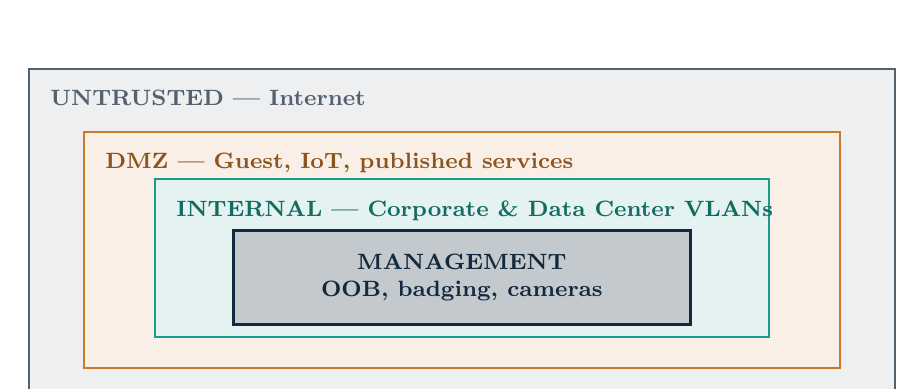
\begin{tikzpicture}[font=\small]
\draw[draw=slategray, thick, fill=slategray!10] (0,0) rectangle (11,4.2);
\node[anchor=north west, font=\bfseries\footnotesize, color=slategray] at (0.15,4.05) {UNTRUSTED --- Internet};

\draw[draw=amber, thick, fill=amber!12] (0.7,0.4) rectangle (10.3,3.4);
\node[anchor=north west, font=\bfseries\footnotesize, color=amber!70!black] at (0.85,3.25) {DMZ --- Guest, IoT, published services};

\draw[draw=teal, thick, fill=teal!12] (1.6,0.8) rectangle (9.4,2.8);
\node[anchor=north west, font=\bfseries\footnotesize, color=teal!70!black] at (1.75,2.65) {INTERNAL --- Corporate \& Data Center VLANs};

\draw[draw=navy, very thick, fill=navy!25] (2.6,0.95) rectangle (8.4,2.15);
\node[font=\bfseries\footnotesize, color=navy, align=center] at (5.5,1.55) {MANAGEMENT\\OOB, badging, cameras};
\end{tikzpicture}
\caption{Nested trust zones: traffic only moves inward or outward through firewall policy, never laterally without inspection.}
\label{fig:zones}
\end{figure}

\section{Firewall Policy Summary}
Table~\ref{tab:policy} summarizes the default posture between zones. All rules are logged;
any traffic not explicitly permitted is denied and alerts on the first match.

\begin{table}[H]
\centering
\rowcolors{2}{palebg}{white}
\begin{tabularx}{\linewidth}{@{}l l X l@{}}
\toprule
\rowcolor{navy}
\thd{Source Zone} & \thd{Destination Zone} & \thd{Allowed Services} & \thd{Action} \\
\midrule
Untrusted   & DMZ          & HTTPS, DNS to published resolvers only & Permit, logged \\
DMZ         & Internal     & None by default & Deny \\
Internal    & DMZ          & HTTPS to published services only & Permit, logged \\
Internal    & Management   & SSH, HTTPS, SNMPv3 from jump hosts only & Permit, logged \\
Management  & Internal     & None outbound except patch mirrors & Permit, logged \\
Untrusted   & Management   & --- & Deny, alert on match \\
\bottomrule
\end{tabularx}
\caption{Default inter-zone firewall policy.}
\label{tab:policy}
\end{table}

% =====================================================================
\chapter{High Availability \& Maintenance}
% =====================================================================

\section{Redundancy Protocols}
First-hop redundancy uses HSRP on all campus and data center distribution pairs, with
priority tuned so the primary distribution switch owns the virtual gateway under normal
conditions and preemption is disabled to avoid unnecessary flapping during brief link blips.

\begin{table}[H]
\centering
\rowcolors{2}{palebg}{white}
\begin{tabularx}{\linewidth}{@{}l l l X@{}}
\toprule
\rowcolor{navy}
\thd{Group} & \thd{Virtual IP} & \thd{Protocol} & \thd{Members} \\
\midrule
HSRP 110 & 10.10.0.1  & HSRPv2 & dist-corp-01 (active), dist-corp-02 (standby) \\
HSRP 120 & 10.10.4.1  & HSRPv2 & dist-corp-01 (active), dist-corp-02 (standby) \\
HSRP 501 & 10.20.1.1  & HSRPv2 & dist-dc-01 (active), dist-dc-02 (standby) \\
VRRP 310 & 172.16.10.1 & VRRPv3 & dist-edge-01 (master), dist-edge-02 (backup) \\
\bottomrule
\end{tabularx}
\caption{First-hop redundancy group assignments.}
\label{tab:hsrp}
\end{table}

\section{Maintenance Window Policy}
\begin{designnote}
Standard maintenance windows run Sundays 01:00--05:00 SGT. Any change touching the core,
security, or edge tiers requires a peer-reviewed rollback plan and a pre-staged
configuration diff attached to the change ticket before the window opens.
\end{designnote}

\section{Monitoring \& Alerting}
\begin{itemize}[leftmargin=1.4em]
  \item BGP session state, OSPF neighbor adjacency, and HSRP/VRRP role changes page the
    on-call engineer within 60 seconds of a state transition.
  \item Interface utilization above 80\% sustained for 5 minutes on any core or edge link
    opens a capacity-planning ticket automatically.
  \item Synthetic transactions verify end-to-end reachability between HQ, DC-East, and
    DC-West every 30 seconds; three consecutive failures trigger failover validation.
\end{itemize}

% =====================================================================
\chapter{Appendix}
% =====================================================================

\section{Glossary}
\begin{description}[leftmargin=3.2em, style=nextline]
  \item[OSPF] Open Shortest Path First --- interior gateway routing protocol used within
    the fabric.
  \item[BGP] Border Gateway Protocol --- exterior routing protocol used with ISP transit
    and the DR site.
  \item[HSRP / VRRP] Hot Standby / Virtual Router Redundancy Protocol --- first-hop gateway
    failover mechanisms.
  \item[DMZ] Demilitarized Zone --- a segregated network exposing services to less-trusted
    networks.
  \item[MLAG] Multi-Chassis Link Aggregation --- allows a pair of switches to present a
    single logical link-aggregation partner to downstream devices.
\end{description}

\section{Revision History}
\begin{table}[H]
\centering
\rowcolors{2}{palebg}{white}
\begin{tabularx}{\linewidth}{@{}l l l X@{}}
\toprule
\rowcolor{navy}
\thd{Version} & \thd{Date} & \thd{Author} & \thd{Summary} \\
\midrule
4.2 & 2026-03-03 & Elena Cho    & Added DC-West DR peering, updated BGP max-prefix limits \\
4.1 & 2025-09-15 & Priya Nair   & Reworked VLAN scheme for guest/IoT separation \\
4.0 & 2025-02-20 & Elena Cho    & Migrated core to MLAG pair, retired legacy STP root \\
3.3 & 2024-07-08 & Marcus Webb  & Added Nairobi branch, corrected supernet table \\
\bottomrule
\end{tabularx}
\caption{Document revision history.}
\label{tab:revhist}
\end{table}

\section{Approval \& Contacts}
\begin{table}[H]
\centering
\rowcolors{2}{palebg}{white}
\begin{tabularx}{\linewidth}{@{}l l X@{}}
\toprule
\rowcolor{navy}
\thd{Role} & \thd{Name} & \thd{Contact} \\
\midrule
Principal Network Architect & Elena Cho   & \faPhone\ ext. 4021 \\
Director of Infrastructure  & Marcus Webb & \faPhone\ ext. 4002 \\
Security Engineering Lead   & Priya Nair  & \faLock\ ext. 4187 \\
Network Operations Center   & On-call rotation & \faServer\ NOC bridge, 24/7 \\
\bottomrule
\end{tabularx}
\caption{Document approval chain and operational contacts.}
\label{tab:contacts}
\end{table}

\end{document}
